\documentclass[tikz,border=4pt]{standalone}
\usepackage[T1]{fontenc}

\usetikzlibrary{positioning,arrows.meta,calc,fit,backgrounds}
\definecolor{ink}{HTML}{0B0B0B}
\definecolor{ink2}{HTML}{52514E}
\definecolor{adj}{HTML}{2A78D6}
\definecolor{adjl}{HTML}{CDE2FB}
\definecolor{pinn}{HTML}{EB6834}
\definecolor{pinnl}{HTML}{FBDCCC}
\definecolor{joint}{HTML}{1BAF7A}
\definecolor{jointl}{HTML}{CDEFE2}
\definecolor{neut}{HTML}{F1F0EC}
\begin{document}
\sffamily
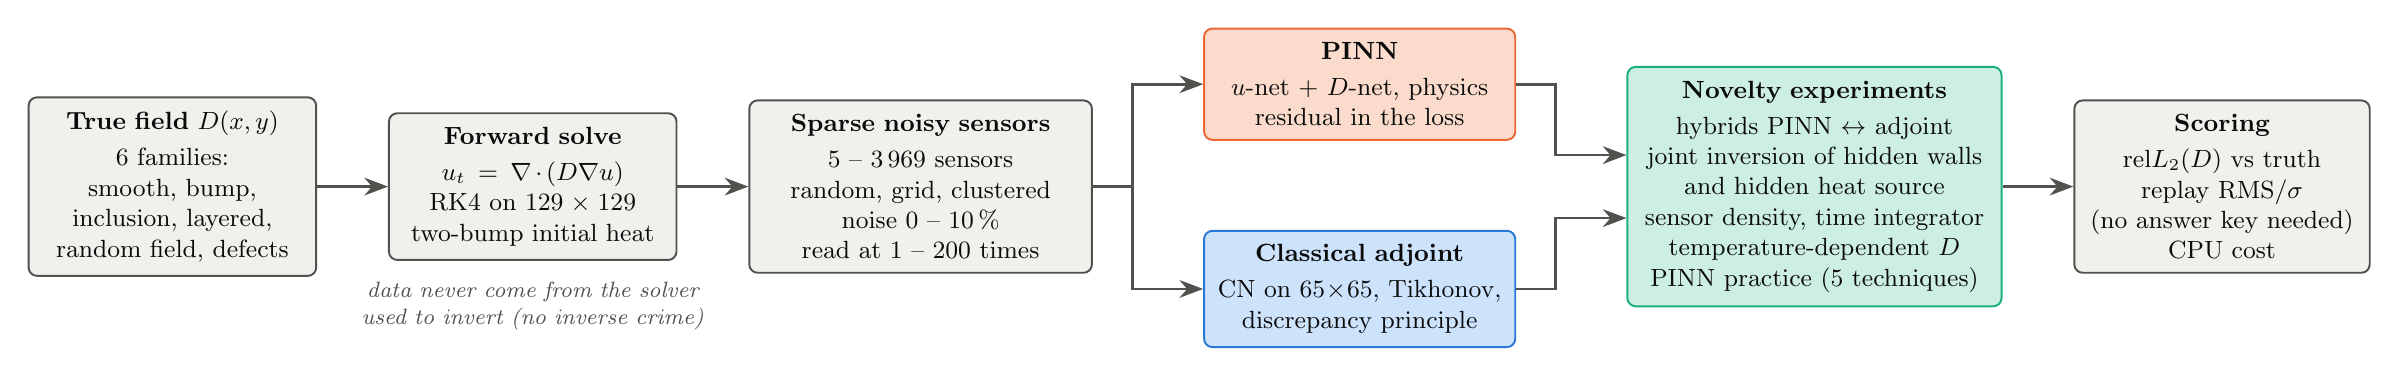
\begin{tikzpicture}[
  node distance=7mm and 9mm,
  box/.style={draw=ink2, line width=0.7pt, rounded corners=3pt, fill=neut, align=center,
              text width=#1, inner sep=5pt, font=\small\color{ink}},
  box/.default=33mm,
  arr/.style={-{Stealth[length=3mm]}, line width=1pt, draw=ink2},
  ttl/.style={font=\small\bfseries}]

\node[box] (truth) {{\bfseries True field $D(x,y)$}\\[2pt]6 families: smooth, bump,\\inclusion, layered,\\random field, defects};
\node[box, right=of truth] (fwd) {{\bfseries Forward solve}\\[2pt]$u_t=\nabla\!\cdot\!(D\nabla u)$\\RK4 on $129\times129$\\two-bump initial heat};
\node[box=40mm, right=of fwd] (sens) {{\bfseries Sparse noisy sensors}\\[2pt]5 -- 3\,969 sensors\\random, grid, clustered\\noise 0 -- 10\,\%\\read at 1 -- 200 times};

\node[box=36mm, fill=pinnl, draw=pinn, right=14mm of sens, yshift=13mm] (pinn) {{\bfseries PINN}\\[2pt]$u$-net + $D$-net, physics\\residual in the loss};
\node[box=36mm, fill=adjl, draw=adj, right=14mm of sens, yshift=-13mm] (adj) {{\bfseries Classical adjoint}\\[2pt]CN on $65\times65$, Tikhonov,\\discrepancy principle};

\node[box=44mm, fill=jointl, draw=joint, right=14mm of pinn, yshift=-13mm] (nov) {{\bfseries Novelty experiments}\\[2pt]
  hybrids PINN $\leftrightarrow$ adjoint\\
  joint inversion of hidden walls\\and hidden heat source\\
  sensor density, time integrator\\
  temperature-dependent $D$\\
  PINN practice (5 techniques)};

\node[box=34mm, right=of nov] (score) {{\bfseries Scoring}\\[2pt]rel$L_2(D)$ vs truth\\replay RMS$/\sigma$\\(no answer key needed)\\CPU cost};

\draw[arr] (truth) -- (fwd);
\draw[arr] (fwd) -- (sens);
\draw[arr] (sens.east) -- ++(5mm,0) |- (pinn.west);
\draw[arr] (sens.east) -- ++(5mm,0) |- (adj.west);
\draw[arr] (pinn.east) -- ++(5mm,0) |- ([yshift=4mm]nov.west);
\draw[arr] (adj.east) -- ++(5mm,0) |- ([yshift=-4mm]nov.west);
\draw[arr] (nov) -- (score);

\node[font=\footnotesize\itshape\color{ink2}, below=1.5mm of fwd, text width=48mm, align=center]
  {data never come from the solver\\used to invert (no inverse crime)};
\end{tikzpicture}
\end{document}
